\documentclass{article}

\usepackage{amsmath}
\usepackage{cleveref}
\usepackage[a4paper,margin=1in]{geometry}
\usepackage{graphicx}
\usepackage{mathtools}
\usepackage{parskip}
\usepackage{rotating}

\title{Black Holes and Accretion Homework}
\author{Calvin Sykes}
\date{\today}

\newcommand{\diff}[1]{\mathrm{d}#1}
\newcommand{\Rin}{\ensuremath R_{\mathrm{in}}}
\newcommand{\mysection}[1]{{\large{\bf #1}}}

\begin{document}

\maketitle

\mysection{Part a)}

The maximum energy that can be liberated by a mass $\diff{m}$ falling onto a black hole with mass $M$ from the innermost stable circular orbit $\Rin$ is given by the mass' potential energy $\diff{U}$:
\begin{equation}
  \label{eq:maxe}
  \diff{U}=-\frac{GM\diff{M}}{\Rin}
\end{equation}

If the mass is in a circular Keplerian orbit at $\Rin$, it has orbital velocity $v=\sqrt{GM/\Rin}$, and so its kinetic energy $T$ is given by:
\begin{equation}
  \label{eq:kine}
  T=\frac{1}{2}\frac{GM\diff{M}}{\Rin}
\end{equation}

Hence, $T=-U/2$, as per the virial theorem. This means that radiating away half of the mass' potential energy will result in its kinetic energy vanishing, and therefore in the mass falling radially into the black hole.

\vspace{\baselineskip}
\mysection{Part b)}

If the mass $\diff{M}$ takes time $\diff{t}$ to fall into the black hole, the accretion rate is $\dot{M}\equiv\diff{M}/\diff{t}$. The rate at which energy is released (i.e. the luminosity) is then:
\begin{equation}
  \label{eq:lum}
  L=\frac{GM\dot{M}}{2\Rin}
\end{equation}

For a Schwarzschild black hole, $\Rin=3R_s$, where $R_s=2GM/c^2$. Hence:
\begin{align}
  L&=\frac{GM}{2}\frac{c^2}{6GM}\dot{M}\\
   &=\frac{c^2}{12}\dot{M}\\
   &=\eta\dot{M}c^2\quad\text{with }\eta=1/12
\end{align}

Similarly, for a maximally rotating black hole with $\Rin=0.6R_s$:
\begin{align}
  L&=\frac{GM}{2}\frac{5c^2}{6GM}\dot{M}\\
   &=\frac{5c^2}{12}\dot{M}\\
   &=\eta\dot{M}c^2\quad\text{with }\eta=5/12
\end{align}

\vspace{\baselineskip}
\mysection{Part c)}

From \cref{eq:maxe}, the radial derivative of the potential energy is:
\begin{equation}
  \label{eq:dUdr}
  \frac{\diff{U}}{\diff{r}}=\frac{GM\diff{M}}{r^2}
\end{equation}

It then follows that the luminosity between $R$ and $R-\diff{R}$ is given by:
\begin{equation}
  \label{eq:lumann}
  L=\frac{GM\dot{M}}{2R^2}\diff{R}
\end{equation}

The area of the annulus with outer (inner) radii of $R$ ($R-\diff{R}$) is:
\begin{equation}
  \label{eq:area}
  A=2\pi R\diff{R}\times 2
\end{equation}

where the factor of 2 is present because both the upper and lower face of the annulus may radiate. Substituting \cref{eq:lumann,eq:area} into the Stefan-Boltzmann law $L=A\sigma_{SB}T^4$ gives:
\begin{equation}
  \label{eq:sb}
  \frac{GM\dot{M}}{2R^2}\diff{R}=4\pi R\diff{R}\sigma_{SB}T^4
\end{equation}

which is the required result.

\vspace{\baselineskip}
\mysection{Part d)}

Definition:
\begin{align}
  L_{\mathrm{edd}}&=4\pi GMm_pc/\sigma_T\\
                  &=\eta\dot{M}_{\mathrm{edd}}c^2
\end{align}

Making the coordinate substitutions $\dot{M}=\dot{m}\dot{M}_{\mathrm{edd}}$ and $R=rR_s$ in \cref{eq:sb}:
\begin{align}
  T^4&=\frac{GM\dot{M}}{8\pi R^3\sigma_{SB}}\\
     &=\frac{GM}{8\pi\sigma_{SB}}\frac{\dot{m}\dot{M}_{\mathrm{edd}}}{r^3{R_s^3}}\\
     &=\frac{GM}{2\sigma_{SB}}\frac{1}{{R_s}^3}\frac{L_{\mathrm{edd}}}{\eta c^2}\frac{\dot{m}}{r^3}\\
     &=\frac{(GM)^2m_p}{2\sigma_{SB}\sigma_T\eta c}\left(\frac{c^2}{2GM}\right)^3\frac{\dot{m}}{r^3}\\
  &=\frac{m_pc^5}{16GM\sigma_{SB}\sigma_T\eta}\frac{\dot{m}}{r^3}
\end{align}

which is the required result.

\vspace{\baselineskip}
\mysection{Part e)}

For a black hole accreting at the Eddington rate, $\dot{m}=1$. The accretion disk temperatures (calculated at $\Rin$) for the four cases requested are then:
\begin{itemize}
    \item $M=10M_\odot$, Schwarzschild ($\Rin=3R_s$): $T=1.24\times 10^7\,\mathrm{K}$
    \item $M=10M_\odot$, maximally spinning ($\Rin=0.6R_s$): $T=2.74\times 10^7\,\mathrm{K}$
    \item $M=10^8M_\odot$, Schwarzschild ($\Rin=3R_s$): $T=2.18\times 10^5\,\mathrm{K}$
    \item $M=10^8M_\odot$, maximally spinning ($\Rin=0.6R_s$): $T=4.87\times 10^5\,\mathrm{K}$
\end{itemize}
\newpage
\begin{sidewaysfigure}[p]
  \centering
  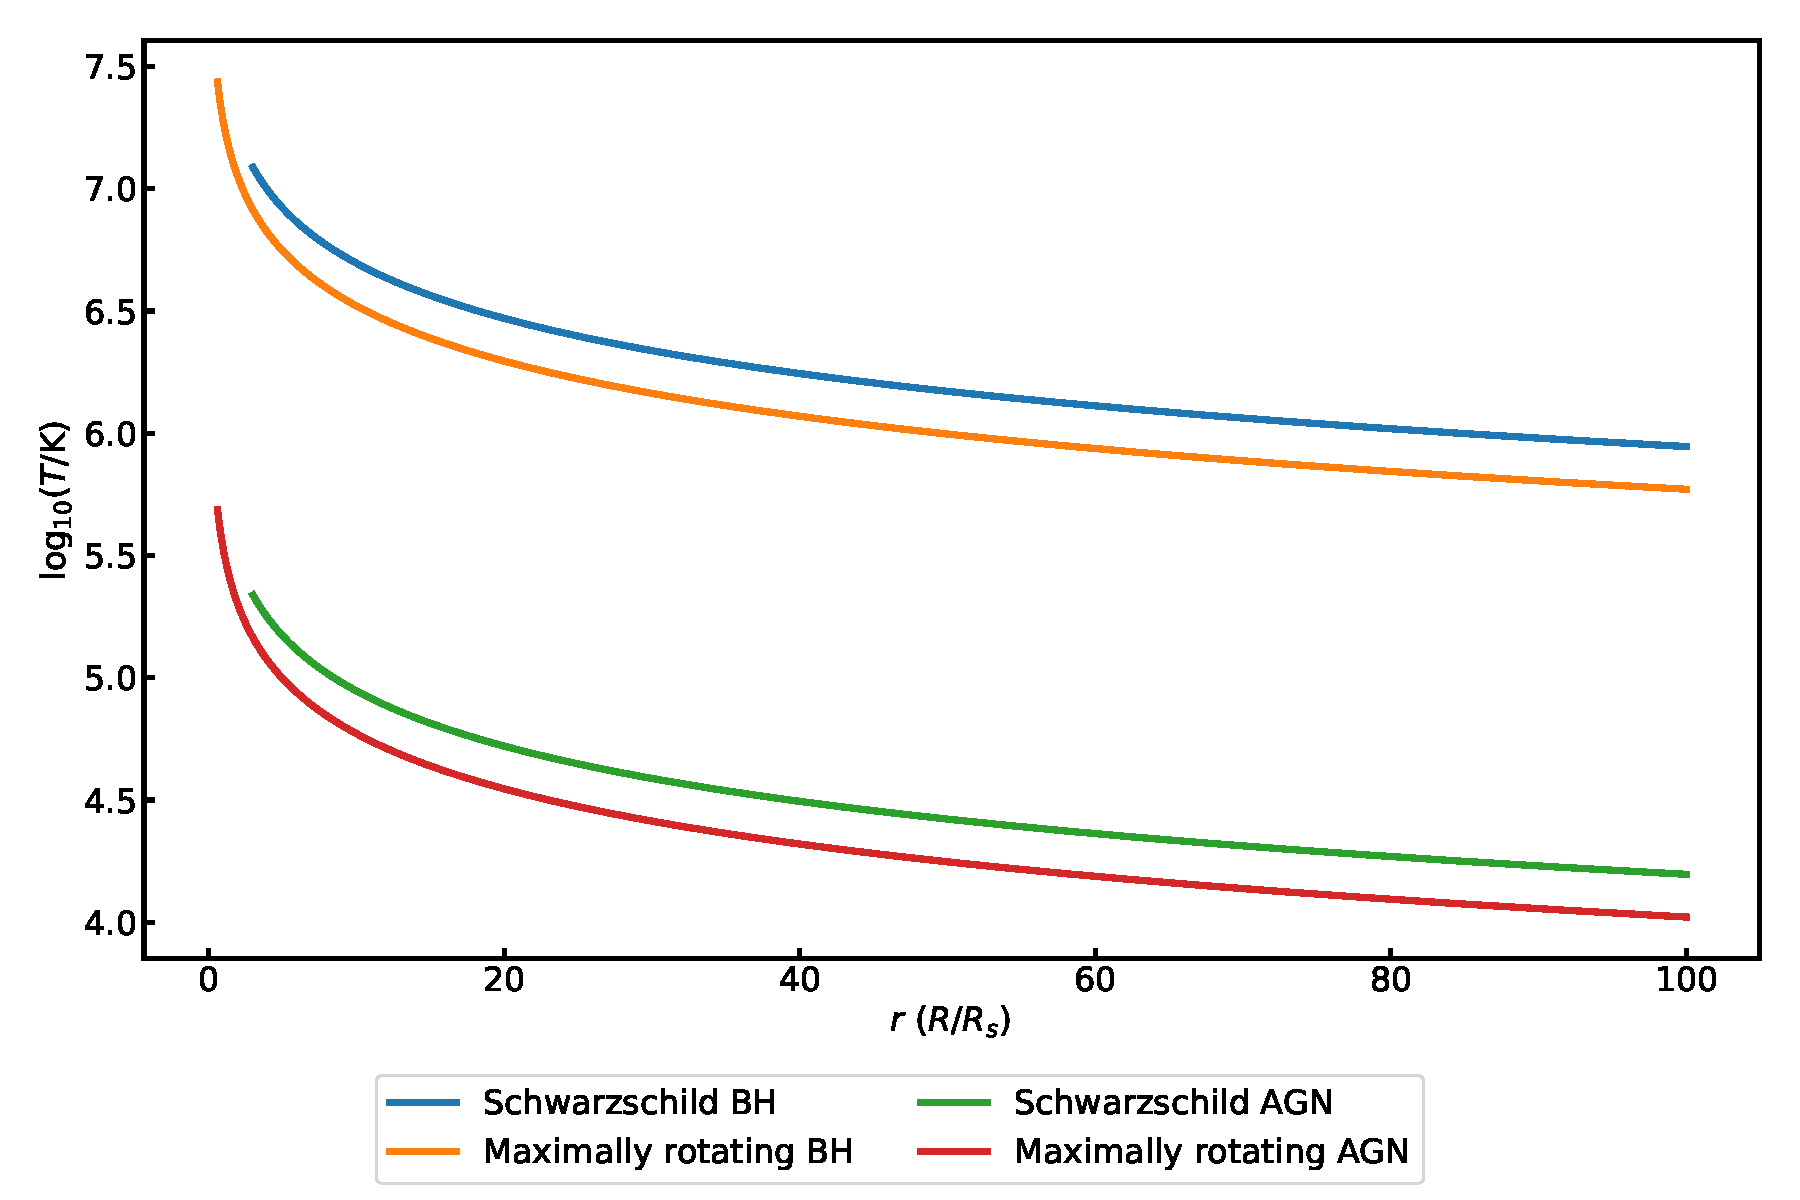
\includegraphics[width=\textwidth]{parte_plot}
\end{sidewaysfigure}
\thispagestyle{empty}

\end{document}